\chapter{Elicitación de requisitos}\label{cap:elicitación_sistema}

\section{Introducción}

La elicitación de requisitos es la base del desarrollo de software, teniendo un gran impacto en las fases posteriores del desarrollo del software. Es a partir de esta elicitación que se obtendrá la información sobre la funcionalidad que se espera de la aplicación.

En este proyecto, al tratar con un cliente real, hemos podido comprobar de primera mano las dificultades que pueden surgir al tratar con una persona que tiene unos conocimientos limitados de informática.


\section{Descripción del sistema actual}

El sistema actual ha sido usado durante bastante tiempo en la vida cotidiana con resultados aceptables. El procedimiento consiste en, mediante el uso de hojas de papel que deben rellenar con los datos a mano, acumular los puntos finales que puedan ser calculados para hallar las posiciones finales de los distintos participantes.

Debido al carácter técnico de la información, los datos, una aplicación genérica no satisface todos los requerimientos de los usuarios. Es por ello por lo que se hace necesario el desarrollo de un sistema específico personalizado a las necesidades del cliente.

\section{Objetivos del sistema}

Este proyecto tiene como objetivo la implementación de un sistema informático que haga uso de una base de datos para almacenar, estudiar y sacar conclusiones sobre los resultados finales de las partidas jugadas, así como facilitar la gestión de las puntuaciones de todos los jugadores y las herramientas físicas necesarias para jugar a dicho juego. Este objetivo general se puede dividir en los siguientes subobjetivos:

\begin{figure}[H]
    \centering
    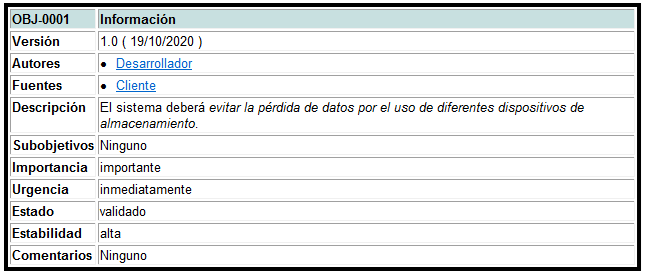
\includegraphics[width=1\linewidth]{fig/Objetivos del sistema/Imagen1.png}
    \caption{Primer objetivo}
    \label{fig:objetivo1}
\end{figure}
\begin{figure}[H]
    \centering
    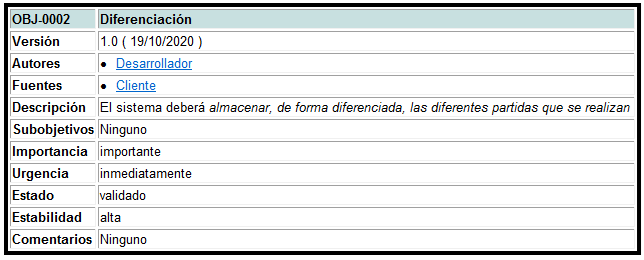
\includegraphics[width=1\linewidth]{fig/Objetivos del sistema/Imagen2.png}
    \caption{Segundo objetivo}
    \label{fig:objetivo2}
\end{figure}
\begin{figure}[H]
    \centering
    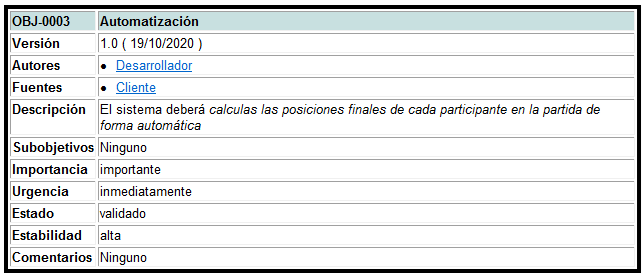
\includegraphics[width=1\linewidth]{fig/Objetivos del sistema/Imagen3.png}
    \caption{Tercer objetivo}
    \label{fig:objetivo3}
\end{figure}
\begin{figure}[H]
    \centering
    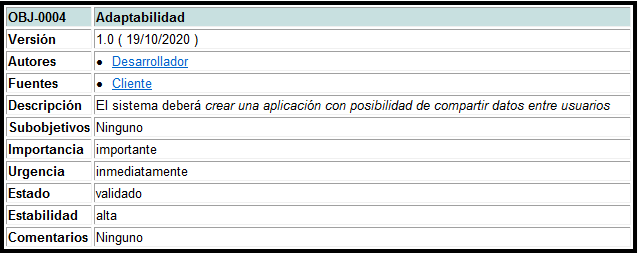
\includegraphics[width=1\linewidth]{fig/Objetivos del sistema/Imagen4.png}
    \caption{Cuarto objetivo}
    \label{fig:objetivo4}
\end{figure}
\begin{figure}[H]
    \centering
    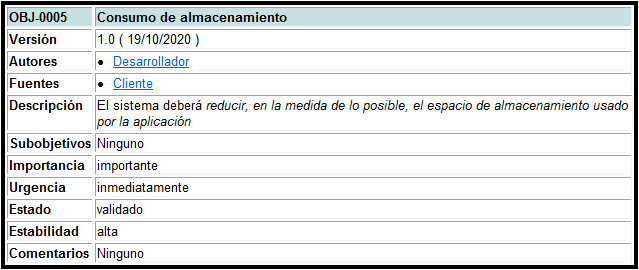
\includegraphics[width=1\linewidth]{fig/Objetivos del sistema/Imagen5.png}
    \caption{Quinto objetivo}
    \label{fig:objetivo5}
\end{figure}

\vspace{1cm}

\section{Requisitos del sistema}

En este apartado desglosaremos detalladamente los requisitos de información, funcionales y no funcionales del sistema. Seguidamente veremos las matrices de rastreabilidad dónde apreciaremos las relaciones entre los requisitos y los objetivos.

\subsection{Requisitos de información}\label{cap:Requisitos del sistema}

\begin{figure}[H]
    \centering
    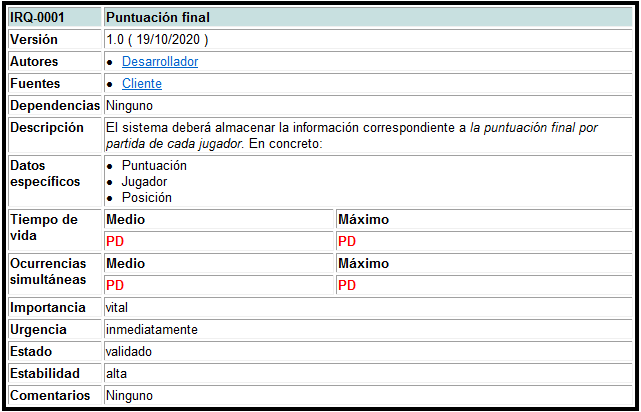
\includegraphics[width=1\linewidth]{fig/Requisitos de información/irq1.png}
    \caption{Primer requisito de información}
    \label{fig:irq1}
\end{figure}
\begin{figure}[H]
    \centering
    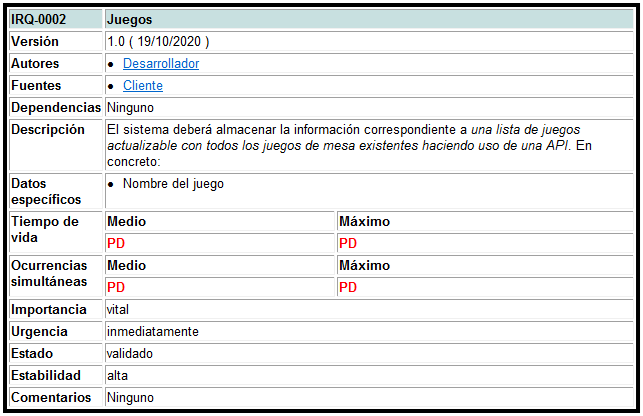
\includegraphics[width=1\linewidth]{fig/Requisitos de información/irq2.png}
    \caption{Segundo requisito de información}
    \label{fig:irq2}
\end{figure}
\begin{figure}[H]
    \centering
    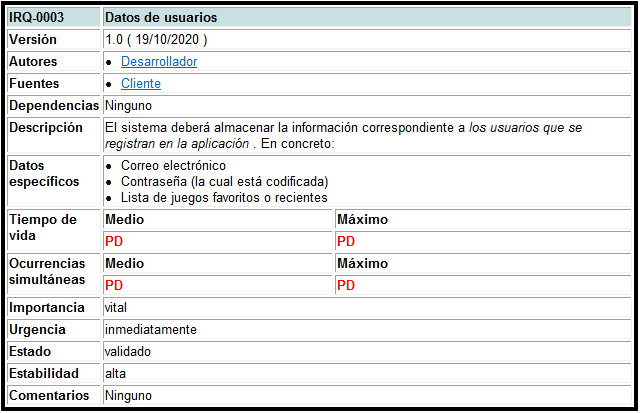
\includegraphics[width=1\linewidth]{fig/Requisitos de información/irq3.png}
    \caption{Tercer requisito de información}
    \label{fig:irq3}
\end{figure}

\subsection{Requisitos funcionales}

\begin{figure}[H]
    \centering
    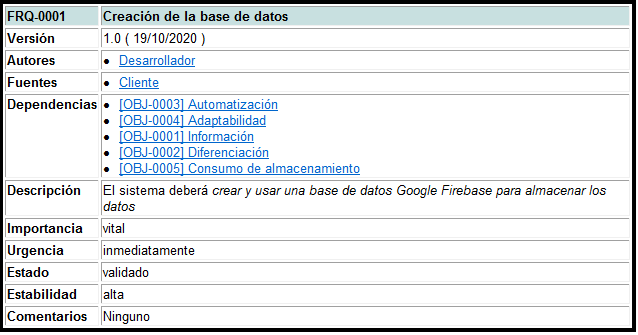
\includegraphics[width=1\linewidth]{fig/Requisitos funcionales/rf1.png}
    \caption{Primer requisito funcional}
    \label{fig:rf1}
\end{figure}
\begin{figure}[H]
    \centering
    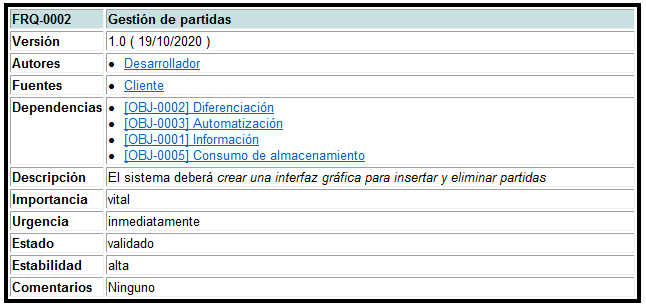
\includegraphics[width=1\linewidth]{fig/Requisitos funcionales/rf2.png}
    \caption{Segundo requisito funcional}
    \label{fig:rf2}
\end{figure}
\begin{figure}[H]
    \centering
    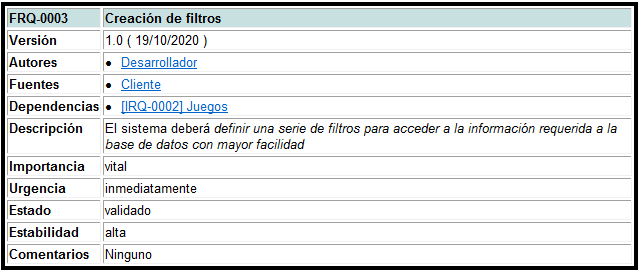
\includegraphics[width=1\linewidth]{fig/Requisitos funcionales/rf3.png}
    \caption{Tercer requisito funcional}
    \label{fig:rf3}
\end{figure}
\begin{figure}[H]
    \centering
    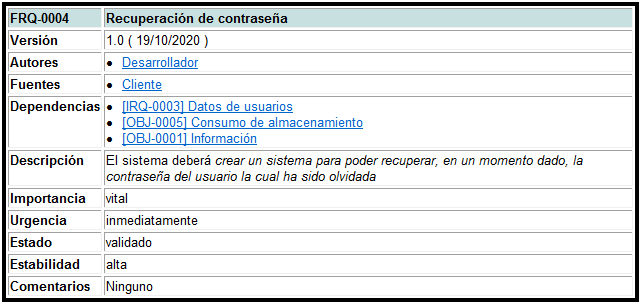
\includegraphics[width=1\linewidth]{fig/Requisitos funcionales/rf4.png}
    \caption{Cuarto requisito funcional}
    \label{fig:rf4}
\end{figure}
\begin{figure}[H]
    \centering
    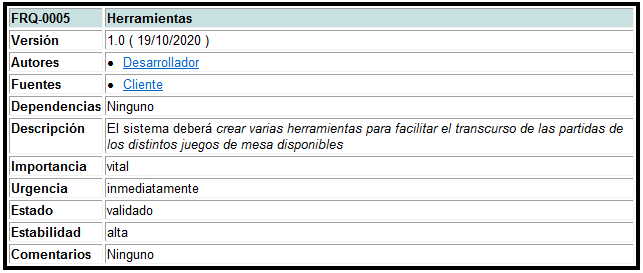
\includegraphics[width=1\linewidth]{fig/Requisitos funcionales/rf5.png}
    \caption{Quinto requisito funcional}
    \label{fig:rf5}
\end{figure}
\begin{figure}[H]
    \centering
    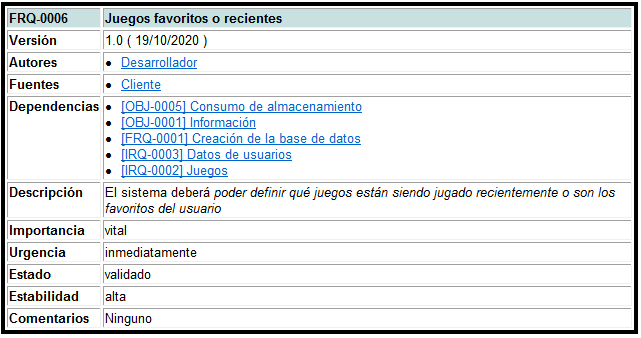
\includegraphics[width=1\linewidth]{fig/Requisitos funcionales/rf6.png}
    \caption{Sexto requisito funcional}
    \label{fig:rf6}
\end{figure}

\subsection{Requisitos no funcionales}

\begin{figure}[H]
    \centering
    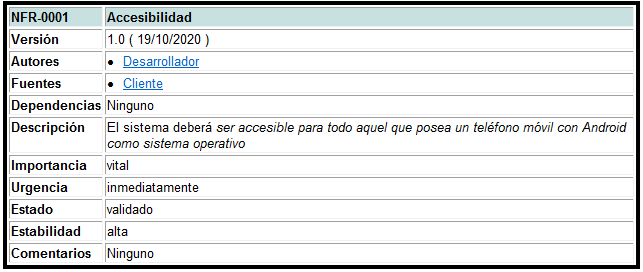
\includegraphics[width=1\linewidth]{fig/Requisitos no funcionales/rnf1.png}
    \caption{Primer requisito no funcional}
    \label{fig:rnf1}
\end{figure}
\begin{figure}[H]
    \centering
    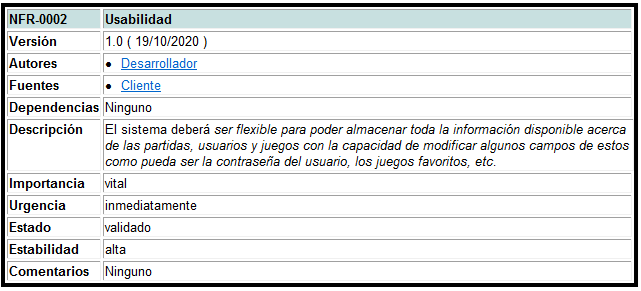
\includegraphics[width=1\linewidth]{fig/Requisitos no funcionales/rnf2.png}
    \caption{Segundo requisito no funcional}
    \label{fig:rnf2}
\end{figure}
\begin{figure}[H]
    \centering
    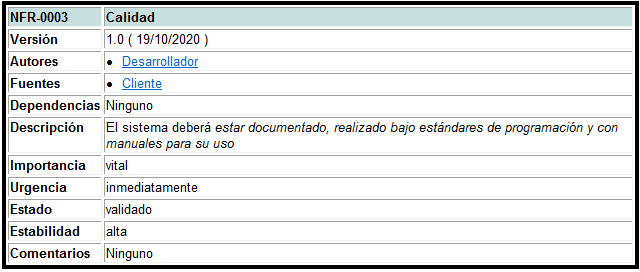
\includegraphics[width=1\linewidth]{fig/Requisitos no funcionales/rnf3.png}
    \caption{Tercer requisito no funcional}
    \label{fig:rnf3}
\end{figure}
\begin{figure}[H]
    \centering
    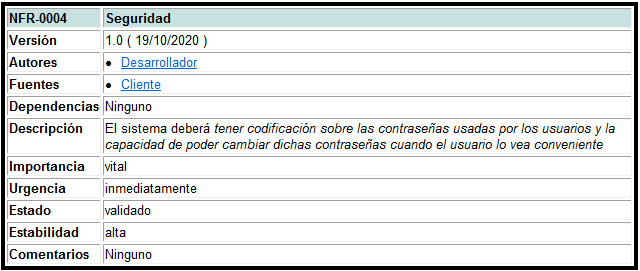
\includegraphics[width=1\linewidth]{fig/Requisitos no funcionales/rnf4.png}
    \caption{Cuarto requisito no funcional}
    \label{fig:rnf4}
\end{figure}
\begin{figure}[H]
    \centering
    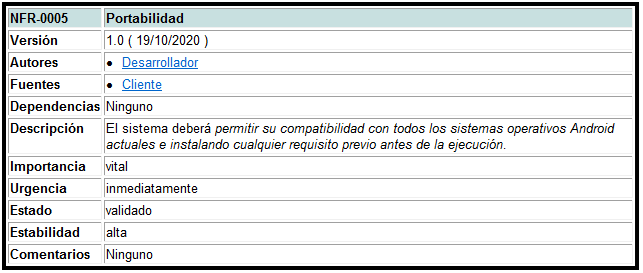
\includegraphics[width=1\linewidth]{fig/Requisitos no funcionales/rnf5.png}
    \caption{Quinto requisito no funcional}
    \label{fig:rnf5}
\end{figure}

\newpage